\section*{Problem Statement}
The problem is to compute the numerical solution of the second-order ordinary differential equation
\[
    m \frac{d^2x}{dt^2} = -k x(t),
\]
where $k > 0$ and $m > 0$, with given initial conditions $x(0) = x_0$, $x'(0) = v_0$. The numerical solution is compared against the exact analytical solution.

\begin{quote}
  \textbf{NOTE}: The code can be accessed using these links: \href{https://raw.githubusercontent.com/HavokSahil/computational-techniques-assignments/refs/heads/main/assignment0/a1_harmonic_osc.m}{MATLAB}, \href{https://raw.githubusercontent.com/HavokSahil/computational-techniques-assignments/refs/heads/main/assignment0/a1_harmonic_osc.jl}{JULIA}
\end{quote}

\section*{Methodology}
The given equation represents the equation of motion of a simple harmonic oscillator. The analytical solution is
\[
    x(t) = A \sin(\omega t + \phi),
\]
where $\omega = \sqrt{\tfrac{k}{m}}$, and $A, \phi$ are determined from the initial conditions.

To compute the numerical solution, the central difference method is used:
\[
    x_{n} = (2 - \tfrac{k \Delta t^2}{m}) x_{n-1} - x_{n-2},
\]
with $x(0) = x_0$ and $x(\Delta t) = x_0 + v_0 \Delta t$.

\subsection*{Pseudo-code}
\begin{enumerate}
    \item Define parameters: $m, k, x_0, v_0, t_{\max}$.
    \item Initialize solution array:
    \begin{align*}
        x(0) &= x_0, \\
        x(\Delta t) &= x_0 + v_0 \Delta t.
    \end{align*}
    \item For $n = 2,3,\dots,N$:
    \[
        x_n = \bigg(2 - \frac{k \Delta t^2}{m}\bigg)x_{n-1} - x_{n-2}.
    \]
    \item Repeat for different values of $\Delta t$.
    \item Compare numerical solutions with analytical solution
    \[
        x(t) = A \sin(\omega t + \phi).
    \]
    \item Plot solution curves and error curves.
\end{enumerate}

\section*{Results}
The following figures illustrate:
\begin{itemize}
    \item The computed solutions for different step sizes $\Delta t$ along with the analytical solution.
    \item The logarithmic absolute deviation of the numerical solutions from the analytical solution.
\end{itemize}

\begin{figure}[h!]
    \centering
    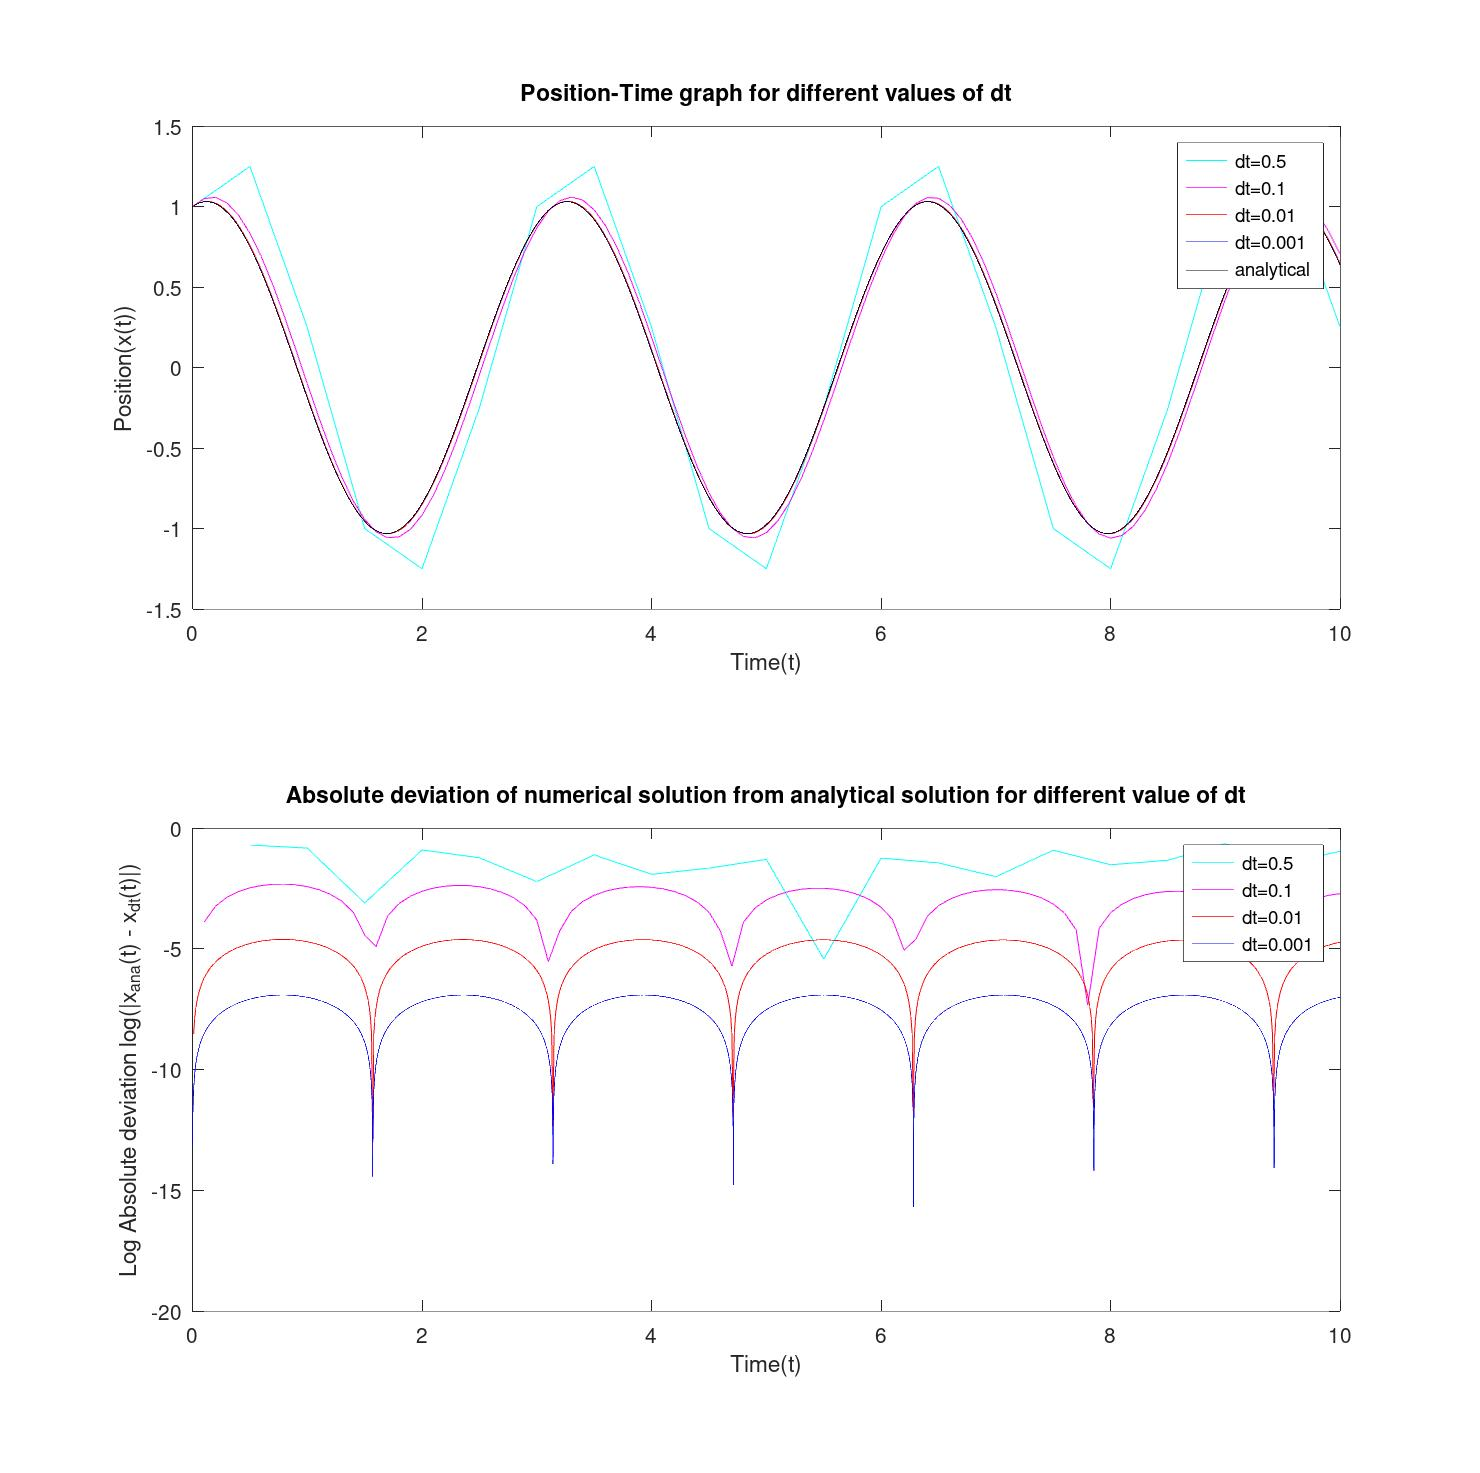
\includegraphics[width=0.75\textwidth]{a3.jpg}
    \caption{Position-time graph for different $\Delta t$ compared with the analytical solution.}
\end{figure}

\section*{Conclusion}
The central difference method provides a stable and accurate approximation of the harmonic oscillator when the time step $\Delta t$ is sufficiently small. Large values of $\Delta t$ lead to noticeable deviations, while smaller steps converge towards the analytical solution. The error plots clearly demonstrate the dependence of accuracy on the step size.
